% pagebreak e pentru a termina de desenat toate pozele inainte...
\pagebreak
\section{Interfața de administrare}

	Interfața de administrare nu poate fi accesată dacă nu se cunoaște ori calea, ori dacă nu se navighează din cadrul vizualizării cererii (pentru client, acest pas reprezintă încărcarea pozelor) pe pagina principală.

	Pagina principală a interfeței de administrare se găsește la:

	\begin{verbatim}
	/admin/
	\end{verbatim}

	În momentul în care utilizatorul navighează la \textit{orice} parte a aplicației de administrare și nu este înregistrat, pagina apare ca în figura~\ref{fig:login}.
	\begin{figure}
		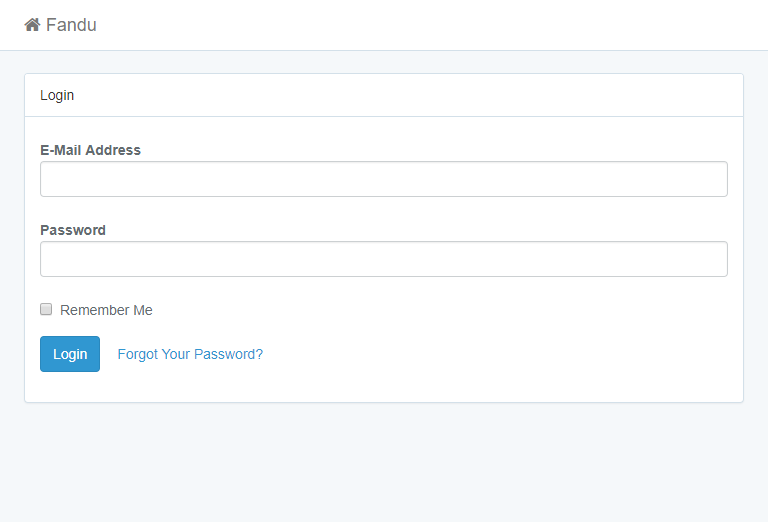
\includegraphics[width=\linewidth]{../imagini/login.png}
		\caption{Pagina de înregistrare pentru interfața de administrare}
		\label{fig:login}
	\end{figure}

	După ce utilizatorul introduce email-ul și parola sa corect în sistem, sistemul va naviga la pagina ce utilizatorul încerca să acceseze.

	Pagina principală a interfeței de administrare arată ca în figura~\ref{fig:home_page}.
	În cazul oricărei probleme, sunt lăsate datele mele de contact pentru a le remedia cât mai rapid.
	De aici, utilizatorul poate introduce rapid un număr de cerere de despăgubire folosind câmpul din bara de navigație.

	În pagina principală, se găsesc două grafice:
	\begin{enumerate}
		\item Primul se referă la cererile de despăgubire noi în această săptămână, raportat la numărul lor pe luna respectivă.
		\item Al doilea se referă la numărul total de decizii terminate, active și refuzate.
	\end{enumerate}

	Numerele folosite în aceste grafice apar atunci când se navighează cu cursorul deasupra lor.

	Bara de navigație conține toate modulele aplicației.

	\begin{figure}
		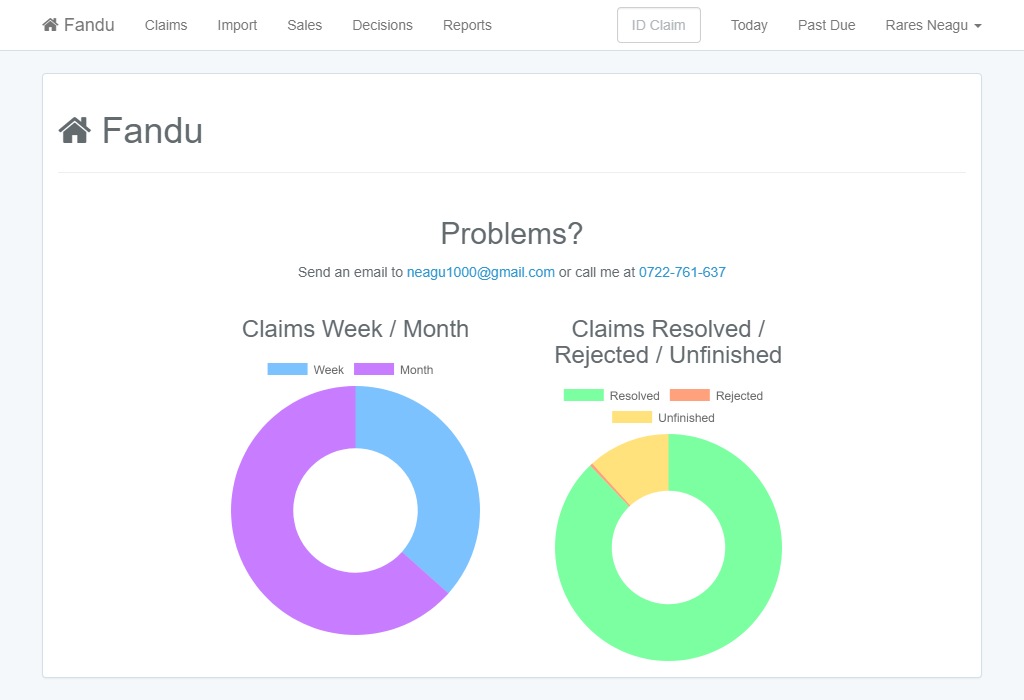
\includegraphics[width=\linewidth]{../imagini/home_page.png}
		\caption{Pagina principală a interfeței de administrare}
		\label{fig:home_page}
	\end{figure}

	\subsection{Modulul cererilor de despăgubire}

	Modulul cererilor de despăgubire se poate accesa prin butonul „Claims” din bara de meniu.

	\begin{figure}
		\subfigure[Structura culorilor] {
			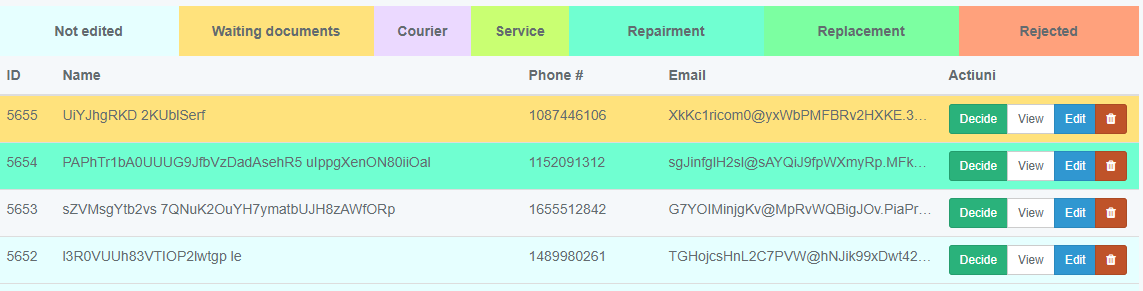
\includegraphics[width=\linewidth]{../imagini/color_coding.png}
			\label{fig:color_coding}
		}
		\subfigure[Filtrarea prin culori] {
			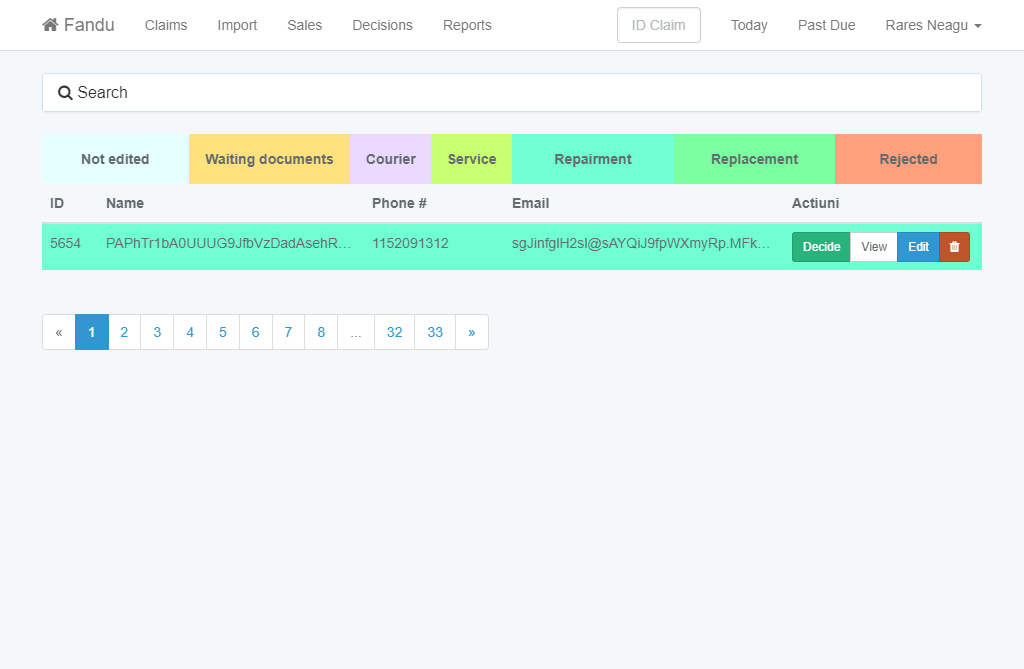
\includegraphics[width=\linewidth]{../imagini/claims_filtered.png}
			\label{fig:claims_filtered}
		}
		\subfigure[Căutarea cererilor] {
			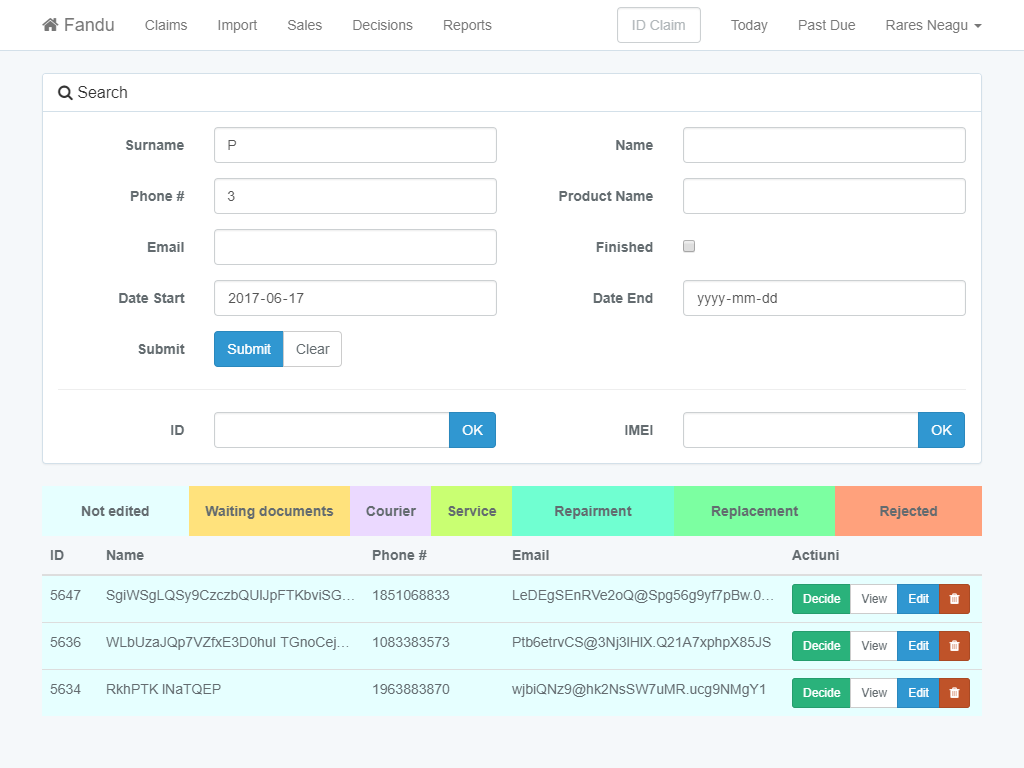
\includegraphics[width=\linewidth]{../imagini/claims_search.png}
			\label{fig:claims_search}
		}
		\subfigure[O cerere cu informații adiționale] {
			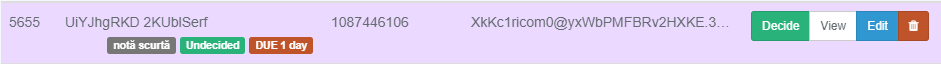
\includegraphics[width=\linewidth]{../imagini/claims_tags.png}
			\label{fig:claims_tags}
		}
		\caption{Interfața administrării cererilor}
	\end{figure}


	Pe pagina principală a modului se vizualizează ultimele 100 cereri de despăgubire în funcție data sosirii lor în sistem.
	Fiecare cerere are patru butoane:
	\begin{enumerate}
		\item \verb|Decide| - pentru a naviga rapid la decizia cererii de despăgubire. Vezi asdasdasd
		\item \verb|View| - vizualizarea cererii de despăgubire scrise de client.
		\item \verb|Edit| - modificarea cererii de despăgubire
		\item \verb|Delete| - iconița de gunoi reprezintă ascunderea cererii din interfața principală.

	\end{enumerate}

	Pentru a ajuta utilizatorul să identifice mai ușor starea cererilor, se reprezintă fiecare linie din tabel cu un sistem de culori, regăsit deasupra capului de tabel.
	Dacă se apasă un element din acesta, se filtrează cererile de pe pagina curentă după elementul respectiv.

	Figura~\ref{fig:color_coding} reprezintă un exemplu a datelor din tabel, figura~\ref{fig:claims_filtered} reprezintă cererile filtrate după „Repairment” (reparare), figura~\ref{fig:claims_search} arată sistemul de căutare în acțiune, iar figura~\ref{fig:claims_tags} prezintă o cerere cu informații adiționale.

	\subsubsection{Vizualizarea și modificarea cererilor}


	Când se vizualizează o cerere, apar date folositoare utilizatorului, conform figurii~\ref{fig:claims_view}, precum:
	\begin{enumerate}
		\item Dacă cererea de despăgubire are un IMEI duplicat cu o altă cerere anterioară de despăgubire.
		\item Dacă nu s-a putut identifica vânzarea, după numărul facturii.
	\end{enumerate}

	\begin{figure}
		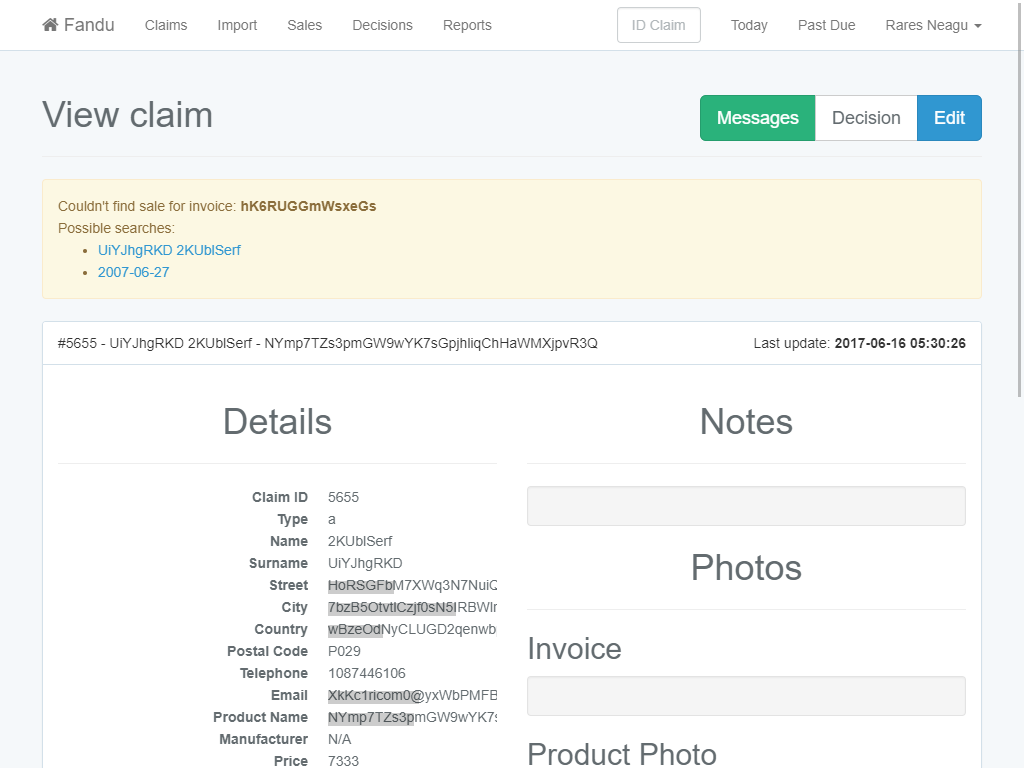
\includegraphics[width=\linewidth]{../imagini/claims_view.png}
		\caption{Date suplimentare pentru utilizator în cadrul vizualizării unei cereri}
		\label{fig:claims_view}
	\end{figure}

	Pentru a modifica cererea, este obligatorie o decizie.
	Utilizatorul nu poate salva niciun câmp, după cum se vede în figura~\ref{fig:claims_edit}.

	După ce se adaugă decizia respectivă, utilizatorul poate scrie un mic detaliu despre cerere, a-i modifica starea, ce implicit modifică și starea deciziei (câmpul „Resolution”) și de a specifica când să-i aducă aminte aplicația despre cerere -- „Reminder” -- pentru a putea fi actualizate.
	Se pot observa aceste câmpuri în figura~\ref{fig:claims_edit_with_decision}.
	\begin{figure}
		\centering
		\subfigure[Fără o decizie - imposibil de modificat] {
			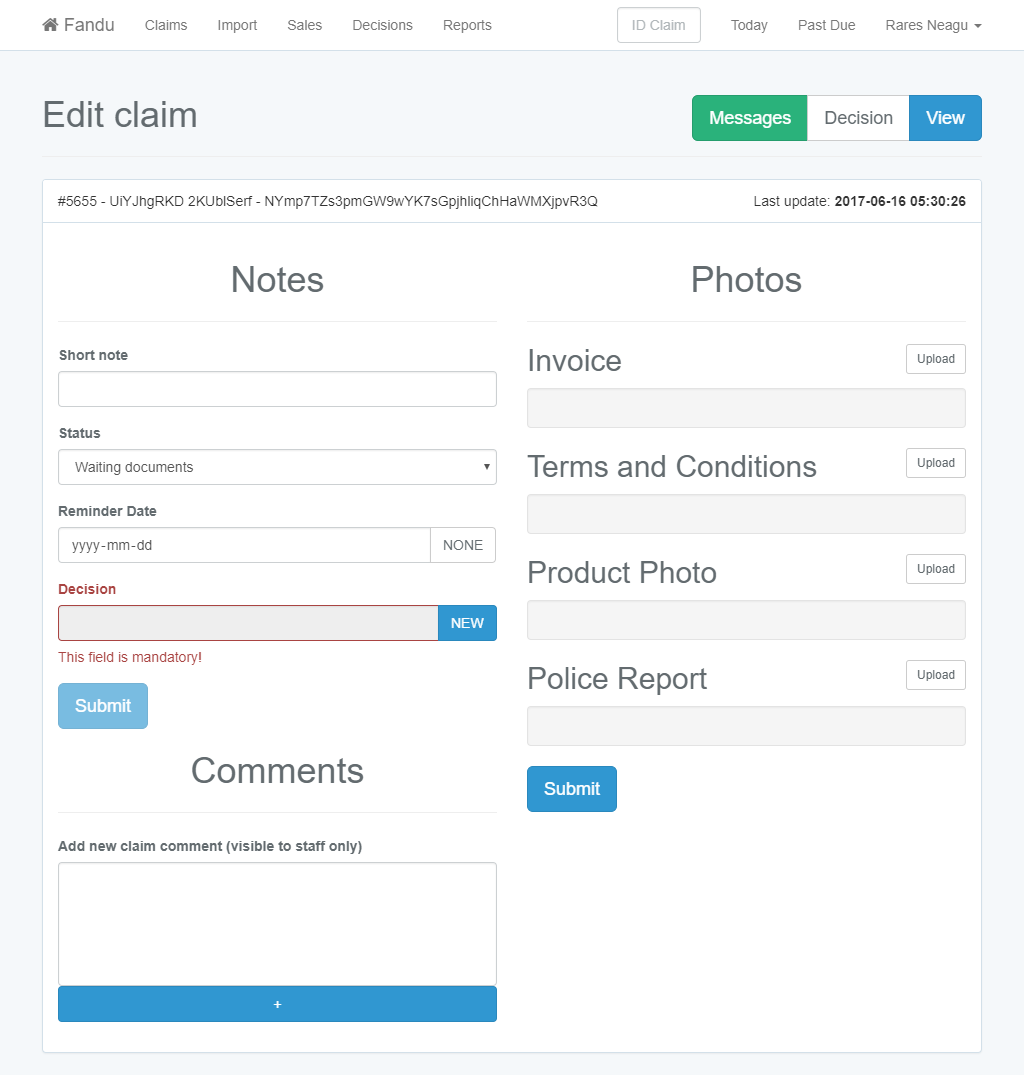
\includegraphics[width=0.4\linewidth]{../imagini/claims_edit.png}
			\label{fig:claims_edit}
		}
		\subfigure[Cu decizie - ușor de modificat] {
			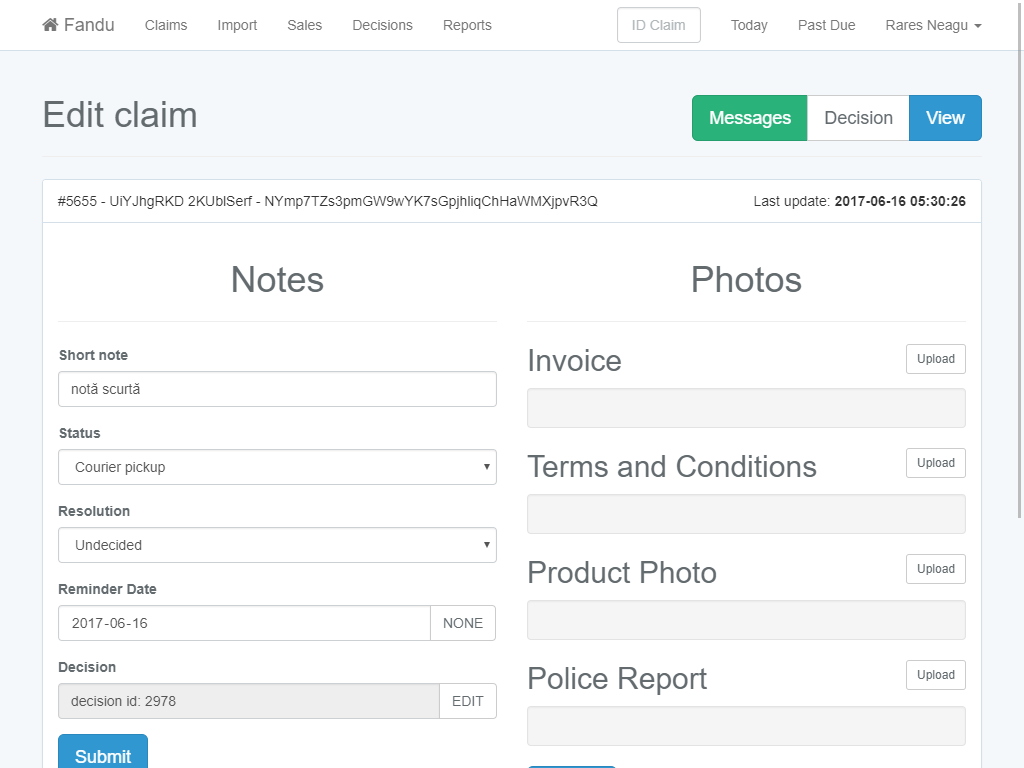
\includegraphics[width=0.4\linewidth]{../imagini/claims_edit_with_decision.png}
			\label{fig:claims_edit_with_decision}
		}
		\caption{Modificarea unei cereri}
	\end{figure}

	\subsubsection{Aducerea aminte a cererilor}

		Pentru că clienții au o perioadă de grație pentru a încărca pozele și pentru că multă lume revine ulterior cu ele, sistemul în meniul principal are două butoane:
		\begin{enumerate}
			\item \verb|Today| - Cererile ce trebuiesc actualizate exclusiv azi.
			\item \verb|Past Due| - Cererile ce trebuiau actualizate, aranjate după când trebuiau actualizate.
		\end{enumerate}
		Ambele secțiuni arată precum figura~\ref{fig:claims_reminders}.
		\begin{figure}
			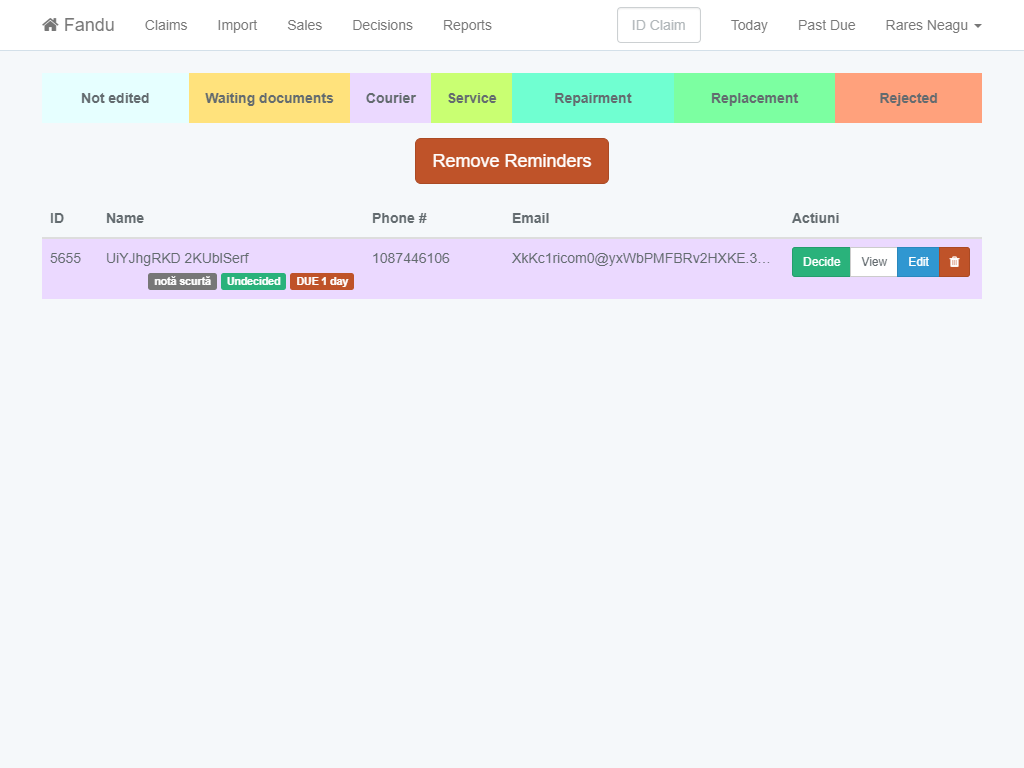
\includegraphics[width=\linewidth]{../imagini/claims_reminder_view.png}
			\caption{Sistemul de aducere aminte a cererilor de despăgubire}
			\label{fig:claims_reminders}
		\end{figure}
		S-a adăugat și butonul de șterge automată a câmpului  „Reminder”.

	\subsection{Modulul introducerii datelor în sistem}

		Introducerea datelor în sistem se face prin butonul „Import” din bara de meniu.
		Apar astfel două panouri, conform figurii~\ref{fig:imports}:
		\begin{enumerate}
			\item \verb|Weekly sale import| - Introducerea raportului principal aplicației. Se va trimite email de confirmare utilizatorilor aplicației, precum cel din~\ref{fig:message_mail_weekly_import}.
			\item \verb|Custom imports| - Introducerea datelor dinaintea aplicării sistemului în funcțiune pentru compania de asigurări.
		\end{enumerate}

		Se vor dezvolta propriile șabloane, ajustate nevoilor fiecărei companii ce folosește acest sistem de gestiune.

		\begin{figure}
			\centering
			\subfigure[Sistemul de introducere a datelor] {
			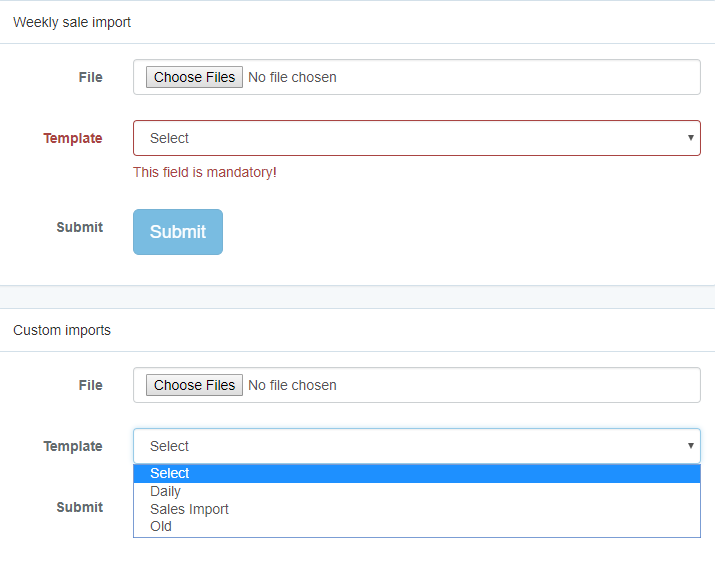
\includegraphics[width=0.6\linewidth]{../imagini/imports.png}
				\label{fig:imports}
			}
			\subfigure[Mesaj trimis utilizatorilor sistemului în momentul adăugării datelor în sistem] {
				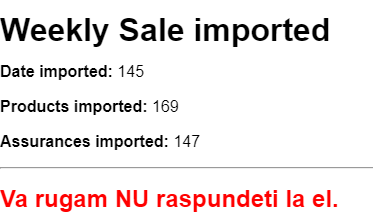
\includegraphics[width=0.2\linewidth]{../imagini/message_mail_weekly_import.png}
				\label{fig:message_mail_weekly_import}
			}
			\caption{Introducerea datelor}
		\end{figure}

		După momentul încărcării, utilizatorul trebuie să aștepte finalizarea introducerii datelor.

		Sistemul are grijă în cazul introducerii unui fișier duplicat, precum se vede în figura~\ref{fig:import_duplicate}, pentru că s-a încercat re-introducerea, din greșeală, aceluiași raport introdus cu succes în figura~\ref{fig:import_great}.

		\begin{figure}
			\centering
			\subfigure[Exemplu la introducerea cu succes a datelor] {
			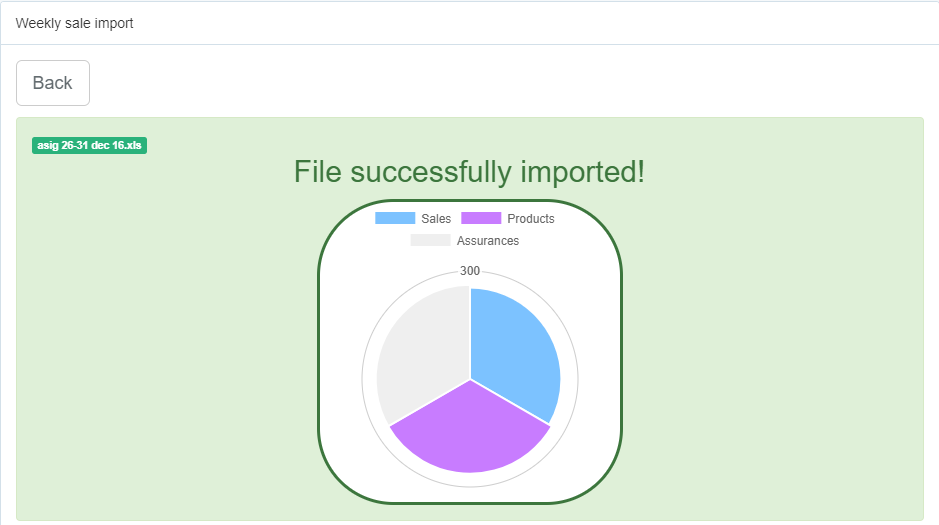
\includegraphics[width=0.4\linewidth]{../imagini/import_great.png}
				\label{fig:import_great}
			}
			\subfigure[Exemplu la încărcarea unui duplicat] {
				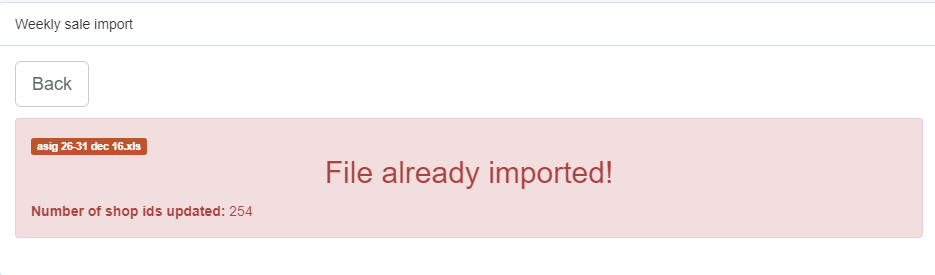
\includegraphics[width=0.4\linewidth]{../imagini/import_duplicate.png}
				\label{fig:import_duplicate}
			}
			\caption{Rezultate posibile la introducerea datelor în sistem}
		\end{figure}

	\subsection{Modulul de vânzări}

		Modulul de vânzări se poate accesa prin butonul „Sales” din bara de meniu.
		Conform figurii~\ref{fig:sales}, sunt afișate într-un tabel vânzările, cu opțiunea de a intra în detalii apăsând pe butonul „View” și de a șterge vânzarea (sau vânzările, dacă se apasă pe butonul „Remove More”) prin apăsarea iconiței în forma unui coș de gunoi.

		Căutarea după numele produsului „Product” sau numele clientului „Customer”, cât și intervalul vânzării produsului se pot vedea în figura~\ref{fig:sales_search}.
		Funcționalitatea este identică pentru momentul legării unei decizii de o vânzare.

	\begin{figure}
		\centering
			\subfigure[Exemplu vânzări] {
				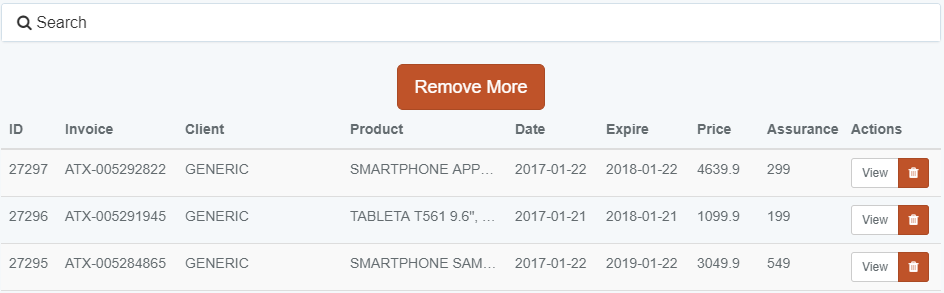
\includegraphics[width=0.4\linewidth]{../imagini/sales.png}
				\label{fig:sales}
			}
			\subfigure[Exemplu căutare vânzări] {
				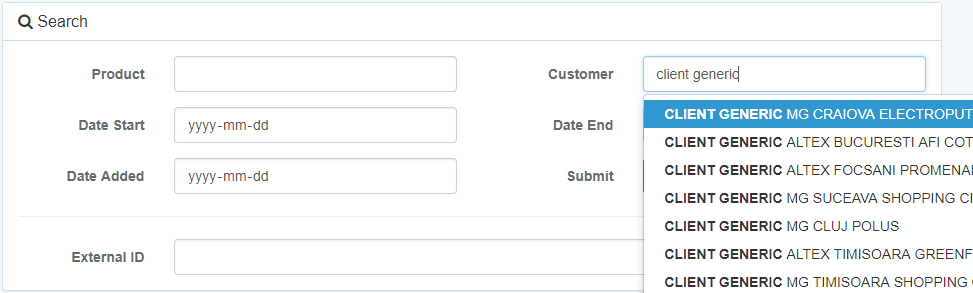
\includegraphics[width=0.4\linewidth]{../imagini/sales_search.png}
				\label{fig:sales_search}
			}
		\caption{Exemplu modul vânzări}
	\end{figure}


		\subsubsection{Vizualizarea vânzării}

			Dacă se apasă pe butonul de vizualizare a unei vânzări, vor apărea din baza de date detaliile vânzării, precum în figura~\ref{fig:sales_view}.

			Din această perspectivă, se pot apăsa următoarele butoane:
			\begin{enumerate}
				\item \verb|Details| - Vizualizarea detaliilor vânzării~\ref{fig:sales_view}.
				\item \verb|Delete Product| - Ștergerea unui produs~\ref{fig:sales_delete_product}
				\item \verb|Delete Assurance| - Ștergerea unei asigurări~\ref{fig:sales_delete_assurance}
				\item \verb|Add Product| - Adăugarea unui produs~\ref{fig:sales_add_product}
				\item \verb|Add Assurance| - Adăugarea unei asigurări~\ref{fig:sales_add_assurance}
			\end{enumerate}
		\begin{figure}
			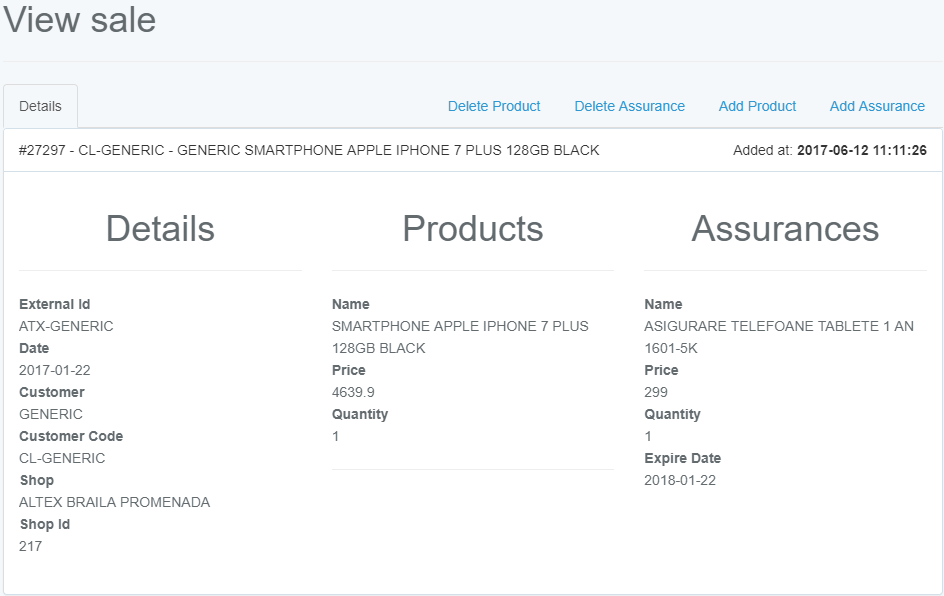
\includegraphics[width=\linewidth]{../imagini/sales_view.png}
			\caption{Detaliile vânzării}
			\label{fig:sales_view}
		\end{figure}
		\begin{figure}
			\centering
			\subfigure[Interfața de adăugare a unei asigurări] {
				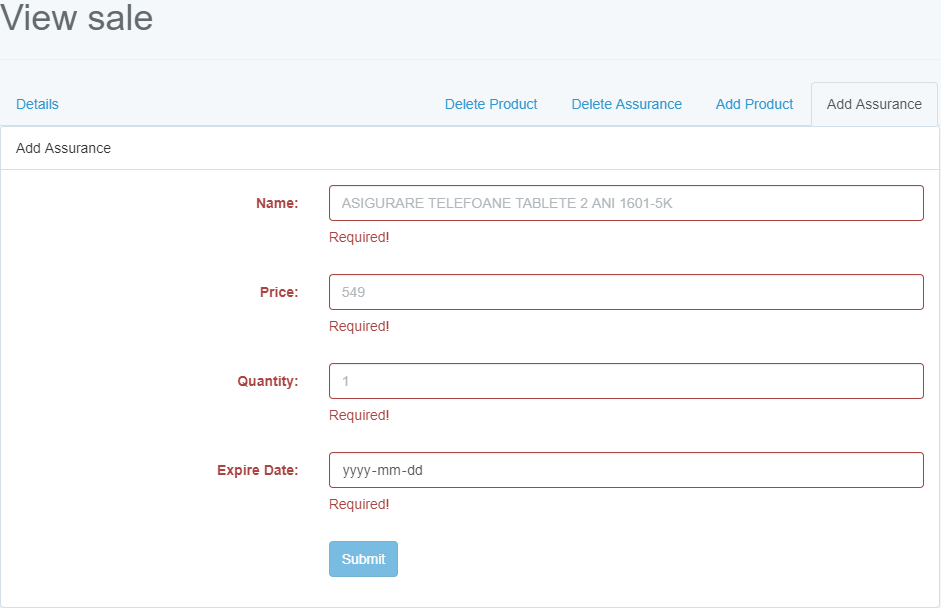
\includegraphics[width=0.4\linewidth]{../imagini/sales_add_assurance.png}
				\label{fig:sales_add_assurance}
			}
			\subfigure[Interfața de adăugare a unui produs] {
				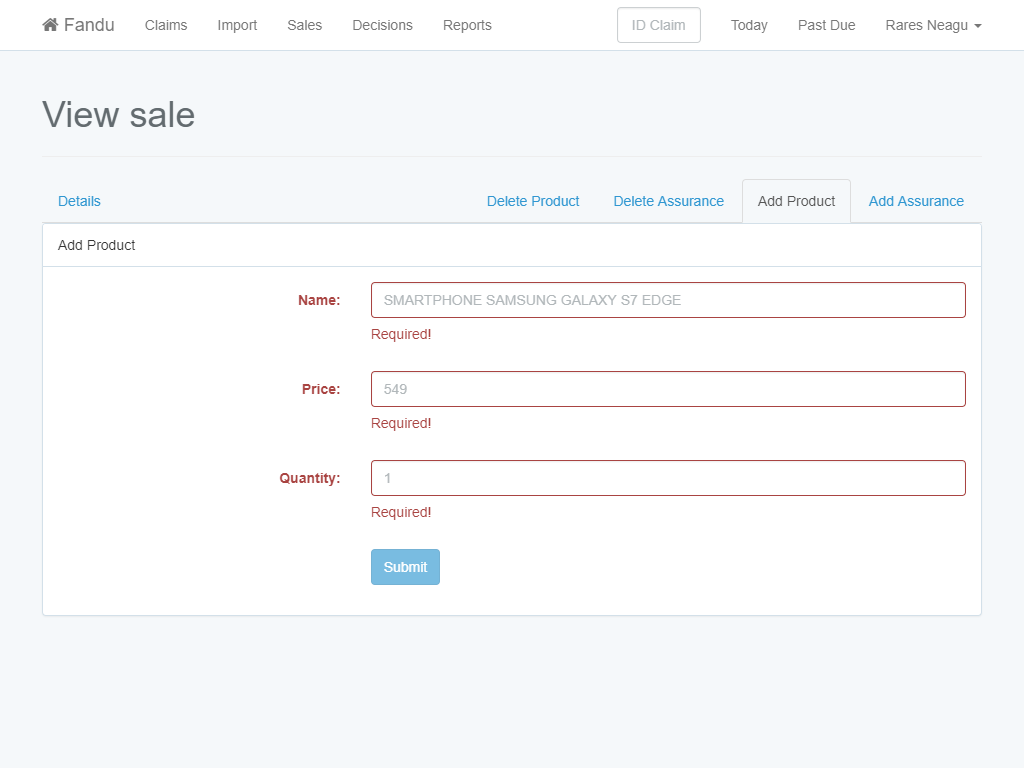
\includegraphics[width=0.4\linewidth]{../imagini/sales_add_product.png}
				\label{fig:sales_add_product}
			}
			\\
			\subfigure[Interfața de ștergere a unei asigurări] {
				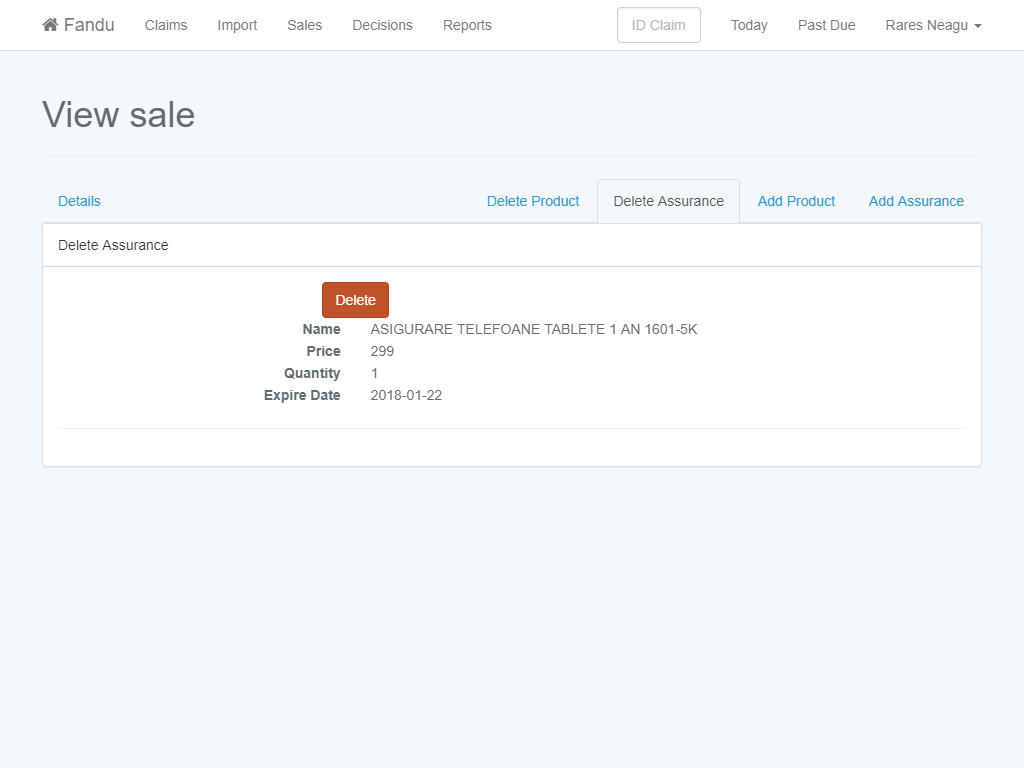
\includegraphics[width=0.4\linewidth]{../imagini/sales_delete_assurance.png}
				\label{fig:sales_delete_assurance}
			}
			\subfigure[Interfața de ștergere a unui produs] {
				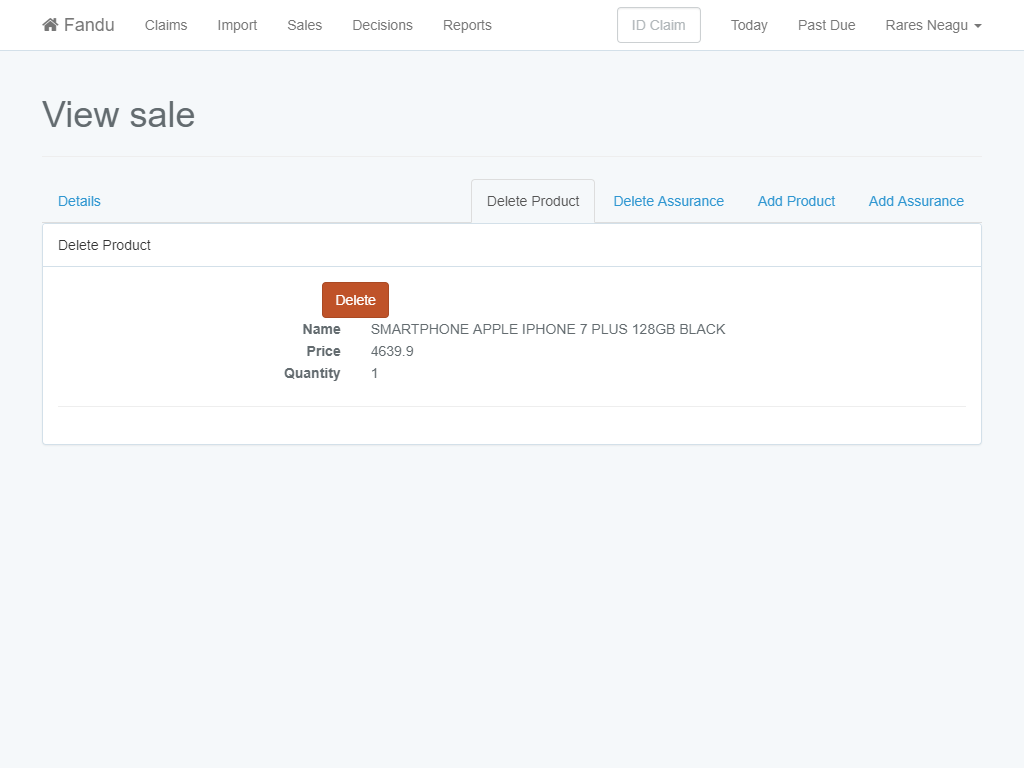
\includegraphics[width=0.4\linewidth]{../imagini/sales_delete_product.png}
				\label{fig:sales_delete_product}
			}
		\caption{Detalii vânzare}
	\end{figure}
	\pagebreak
	\subsection{Crearea unei decizii}

		Crearea unei decizii se face apăsând butonul „Decision” în cadrul vizualizării tabelului cererilor sau vizualizării / modificării unei cereri.

		În care nu există, se va crea o nouă decizie urmărind următorii pași:
		\begin{enumerate}
			\item Dacă se poate găsi automat o vânzare în funcție de numărul facturii, se va sări pasul~\ref{itm:asociere_manuala} și se va trece la pasul~\ref{itm:asociere_vanzare}.
			\item
			Dacă nu se poate găsi automat o vânzare, se va afișa pagina de asociere manuală a vânzării, precum în figura~\ref{fig:claims_match_sale}.
			\label{itm:asociere_manuala}
			\item Dacă nu se poate găsi vânzarea, se poate apăsa butonul „Manual Sale”, de a introduce manual valorile necesari construirii deciziei, precum în figura~\ref{fig:claims_manual_sale}.

			Acest pas este ultimul în cazul construirii legăturii manuale.

			\item Ecranul va arăta precum în figura~\ref{fig:claims_match_confirm}, pentru a valida produsul și asigurarea asociată vânzării.
			\label{itm:asociere_vanzare}
		\end{enumerate}

	\begin{figure}
		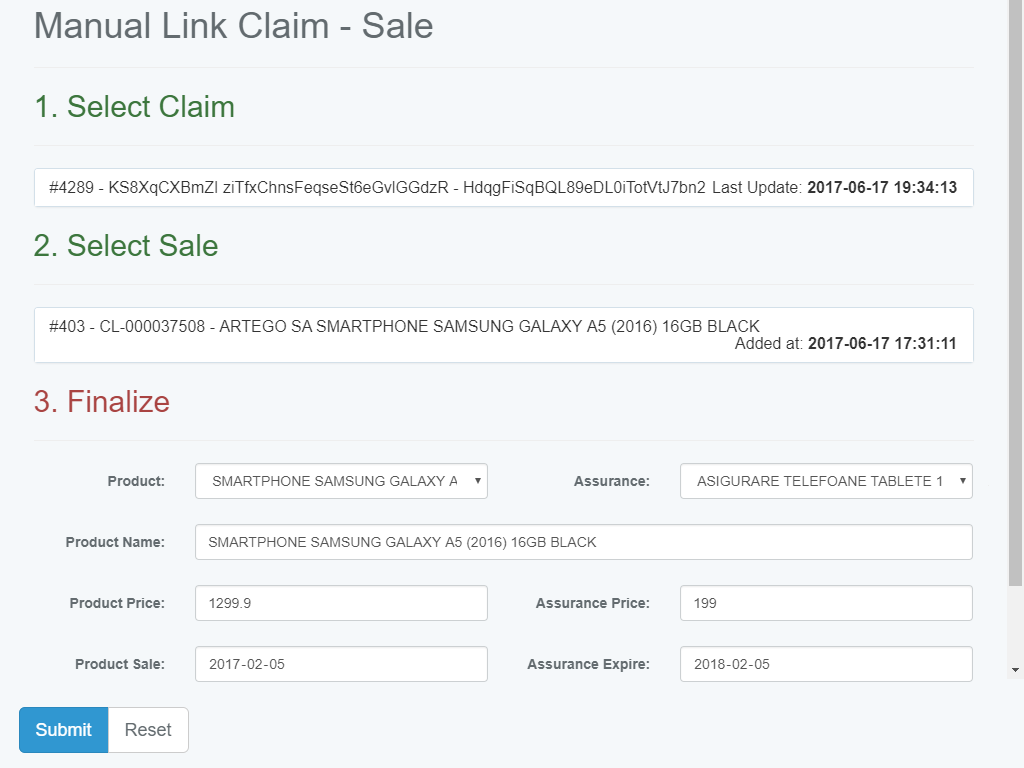
\includegraphics[width=\linewidth]{../imagini/claims_match_confirm.png}
		\caption{Confirmarea legăturii între cerere și vânzare}
		\label{fig:claims_match_confirm}
	\end{figure}

	\begin{figure}
		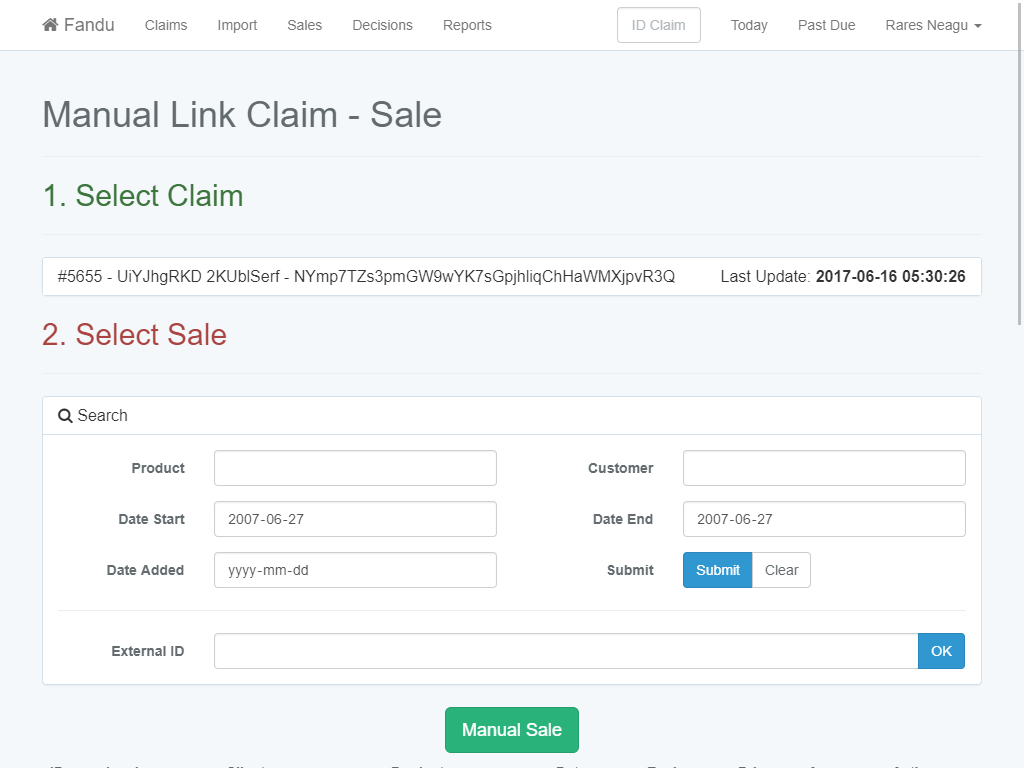
\includegraphics[width=\linewidth]{../imagini/claims_match_sale.png}
		\caption{Selectarea manuală a vânzării}
		\label{fig:claims_match_sale}
	\end{figure}

	\begin{figure}
		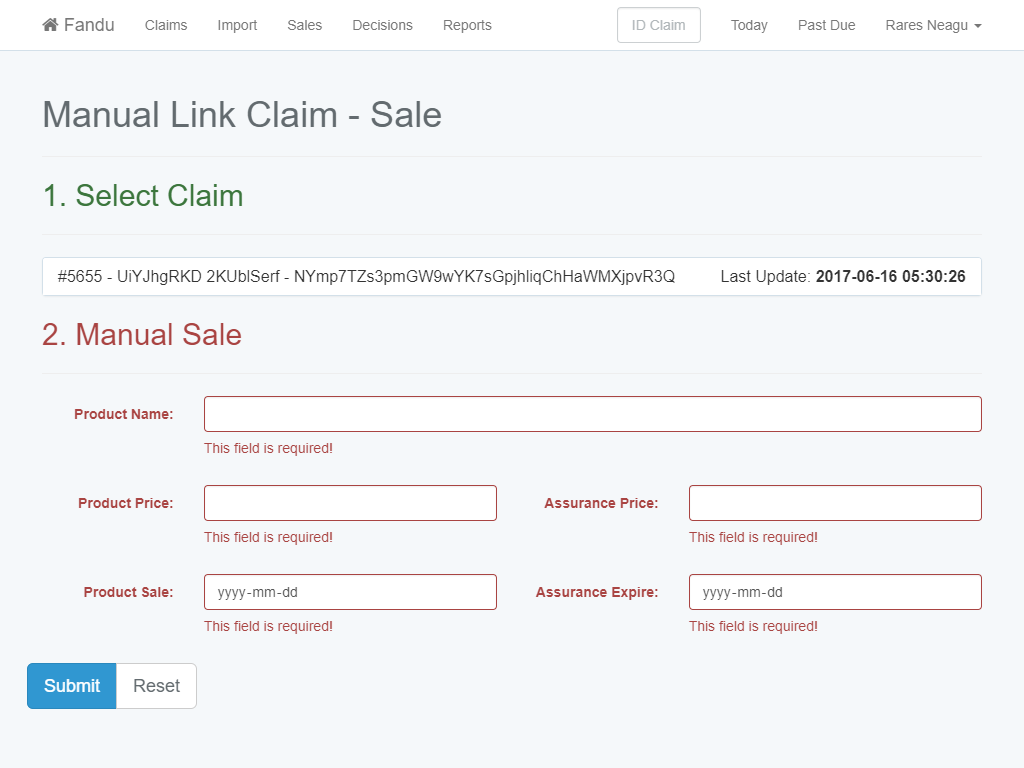
\includegraphics[width=\linewidth]{../imagini/claims_manual_sale.png}
		\caption{Construirea manuală a vânzării}
		\label{fig:claims_manual_sale}
	\end{figure}


	\subsection{Modulul de decizii}

		Modulul de decizii se poate accesa prin butonul „Decision” din bara de meniu.
		Conform figurii~\ref{fig:decisions_filter}, sunt afișate într-un tabel deciziile, cu opțiunea de a intra în detalii apăsând pe butonul „View” și de a șterge decizia prin apăsarea iconiței în forma unui coș de gunoi.
		Opțiunea de a șterge decizia există pentru a se putea reface aceasta în cazul alegerii unei vânzări proaste.

		De asemenea, la fel ca la modulul de vânzări, se reprezintă fiecare linie din tabel cu un sistem de culori, regăsit deasupra capului de tabel.
		Dacă se apasă un element din acesta, se filtrează cererile de pe pagina curentă după elementul respectiv.

		Căutarea se pot vedea în figura~\ref{fig:sales_search}.
		Este o combinație între căutarea vânzării și a datelor aflate în decizie.
		Căutarea după dată caută momentul construirii deciziei.
		Funcționalitatea este identică când se dorește adăugarea unei decizii soluționate anterior în cadrul „Add Old Decision”, când se modifică decizia vizualizată.

		\begin{figure}
			\centering
				\subfigure[Exemplu decizii deja filtrate după condiția de a fi reparate] {
					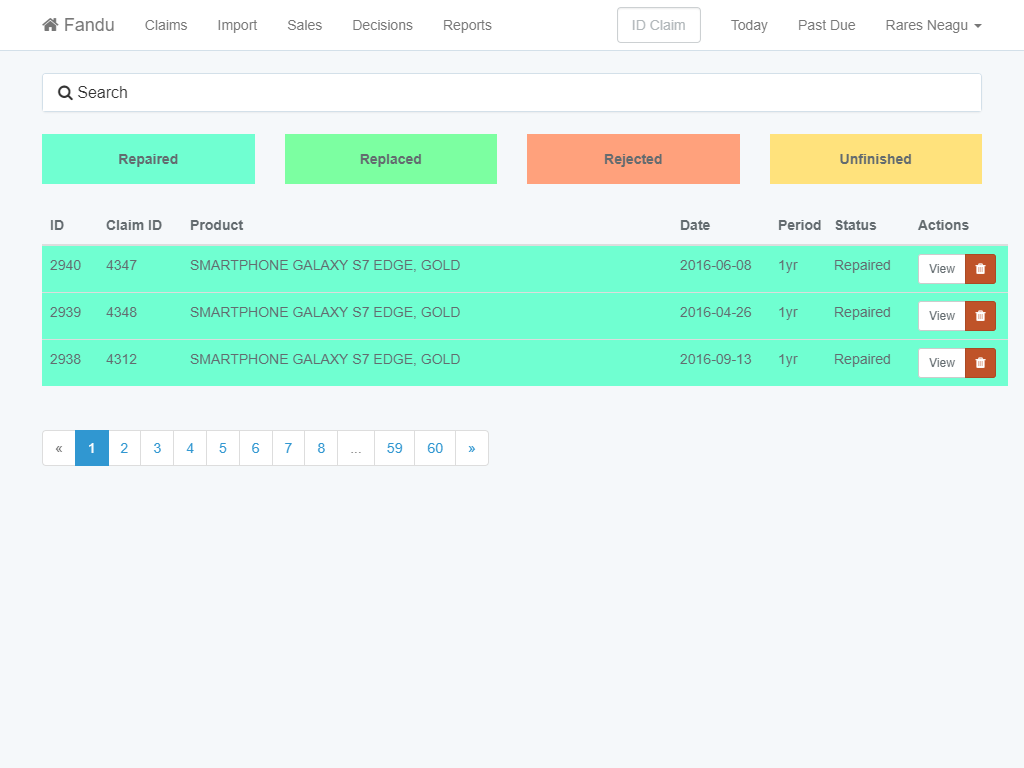
\includegraphics[width=0.4\linewidth]{../imagini/decisions_filter.png}
					\label{fig:decisions_filter}
				}
				\subfigure[Exemplu căutare decizii] {
					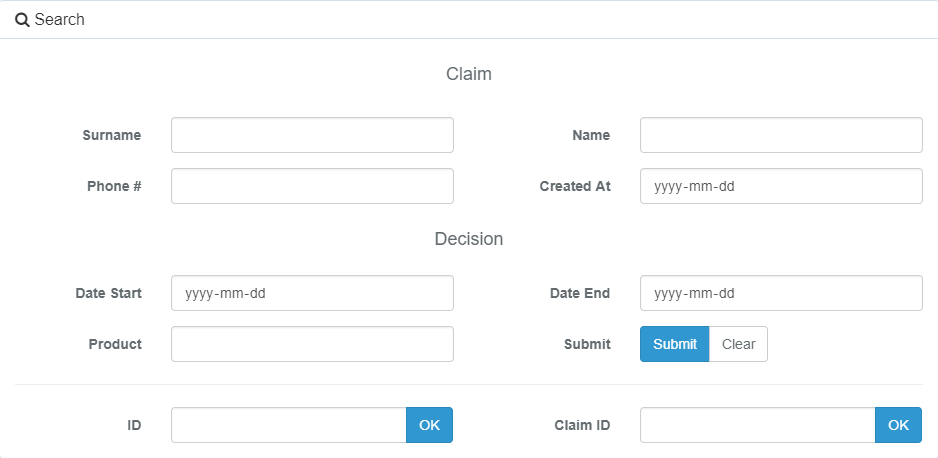
\includegraphics[width=0.4\linewidth]{../imagini/decisions_search.png}
					\label{fig:decisions_search}
				}
			\caption{Exemplu modul vânzări}
		\end{figure}

		\subsubsection{Modificarea deciziilor}

			Interfața de modificare a deciziilor se regăsește la figura~\ref{fig:decisions_edit}.
			Se navighează la cerere, vânzare sau mesaje, dar se poate și adăuga o decizie soluționată deja, pentru a calcula automat ce valoare a rămas acoperită pentru repararea produsului pentru polița de asigurare respectivă, folosind următoarele butoane:
			\begin{enumerate}
				\item \verb|Decision| - Navigarea la detaliile deciziei, vizibilă în momentul încărcării paginii.
				\item \verb|Claim| - Vizualizarea cererii de despăgubire.
				\item \verb|Messages| - Vizualizarea mesajelor interschimbate de utilizatorii aplicației și client.
				\item \verb|Add Old Decision| - Adăugarea deciziilor soluționate anterioare.
				Pentru această interfață se poate vizualiza figura~\ref{fig:decisions_add_old}.
				După ce se selectează decizia anterioară, trebuie confirmată conform figurii~\ref{fig:decisions_add_conirm} înainte de a fi introdusă legătura în baza de date.
				\item \verb|Edit Claim| - Legătură rapidă către modificarea datelor cererii de despăgubire.
				Acest buton a fost adăugat în urma analizei funcționării programului de către utilizatori.
			\end{enumerate}

			Următoarele câmpuri sunt calculate automat și nu pot fi modificate:
			\begin{itemize}
				\item \verb|Client Price To Pay| - Valoarea de plătit de către client, în cazul care nu este acoperită total repararea sau înlocuirea telefonului de polița de asigurare.
				\item \verb|Franchise| - În cazul înlocuirii telefonului, franciza se calculează automat în funcție de prețul telefonului.
				\item \verb|Net Payable| - Suma de plătit către firma de asigurare de operatorii sistemului de gestiune a cererilor de despăgubire.
			\end{itemize}
			\label{lst:itemize}

			Dacă soluția este să se înlocuiască produsul (conform câmpului „Resolution”), se va ascunde câmpul \\
			\verb|Repair / Replace Cost|, pentru că suma de înlocuit produsul va fi prețul din câmpul \verb|Payee Cost|.

			În partea de jos a paginii se găsește un calculator interactiv, ce lasă utilizatorul să vadă estimarea câmpurilor calculate automat, conform listei \hyperref[lst:itemize]{de mai sus}.

			\begin{figure}
				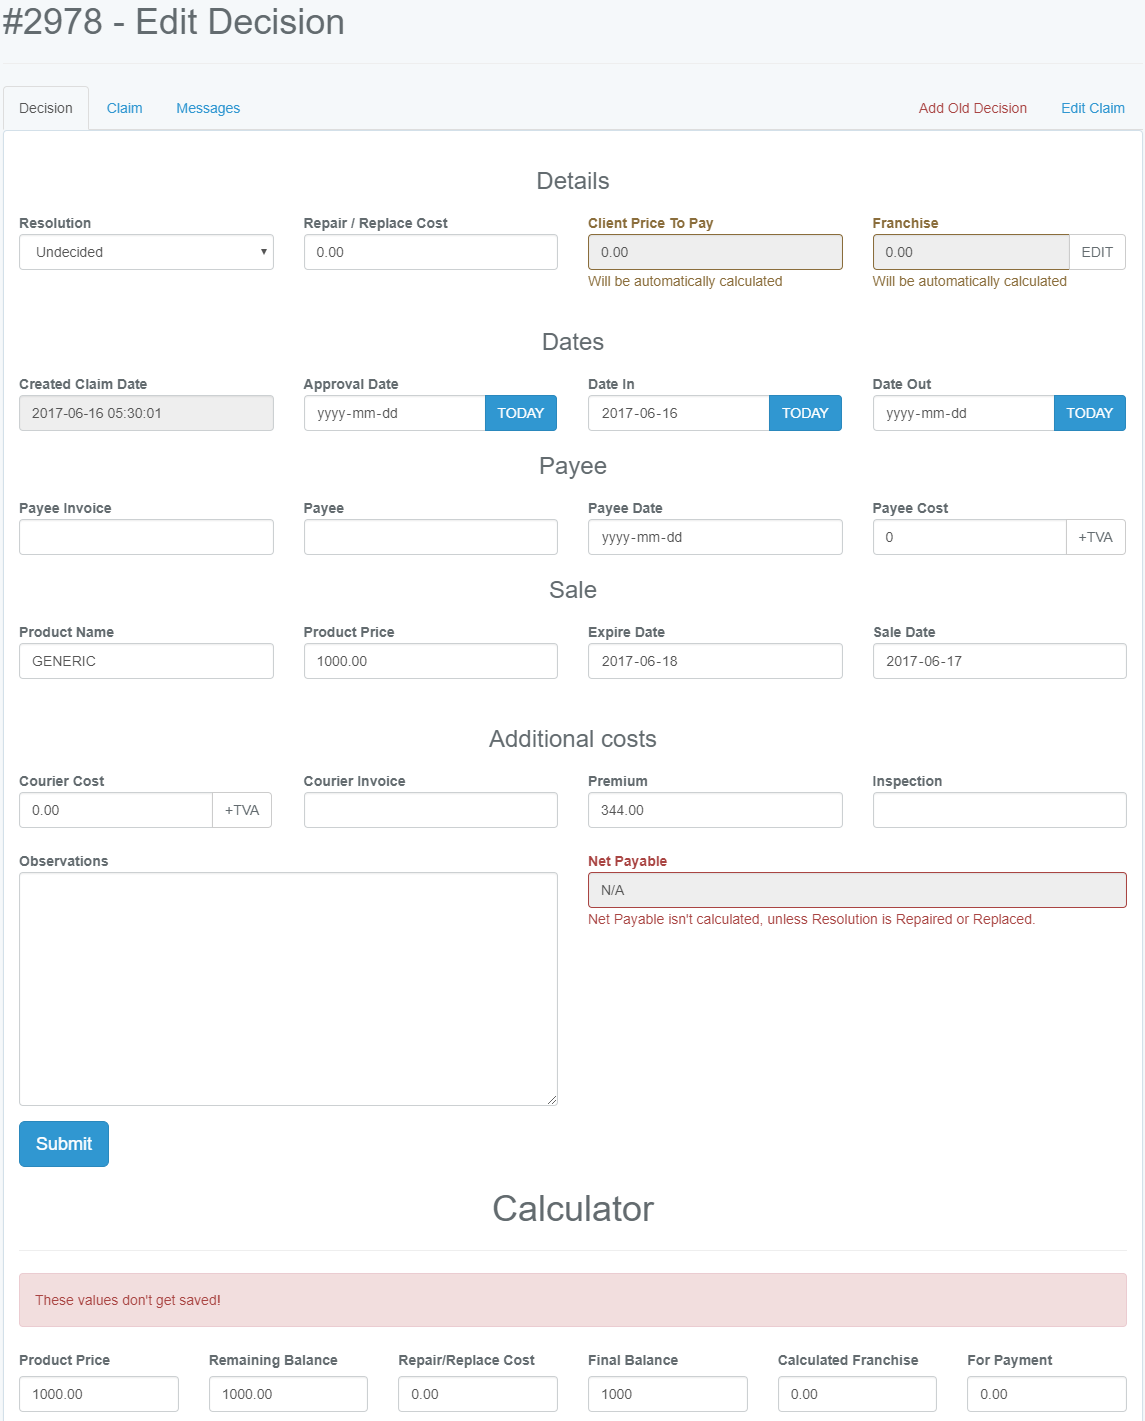
\includegraphics[width=\linewidth]{../imagini/decisions_edit.png}
				\caption{Interfața de modificare a deciziilor}
				\label{fig:decisions_edit}
			\end{figure}


		\begin{figure}
			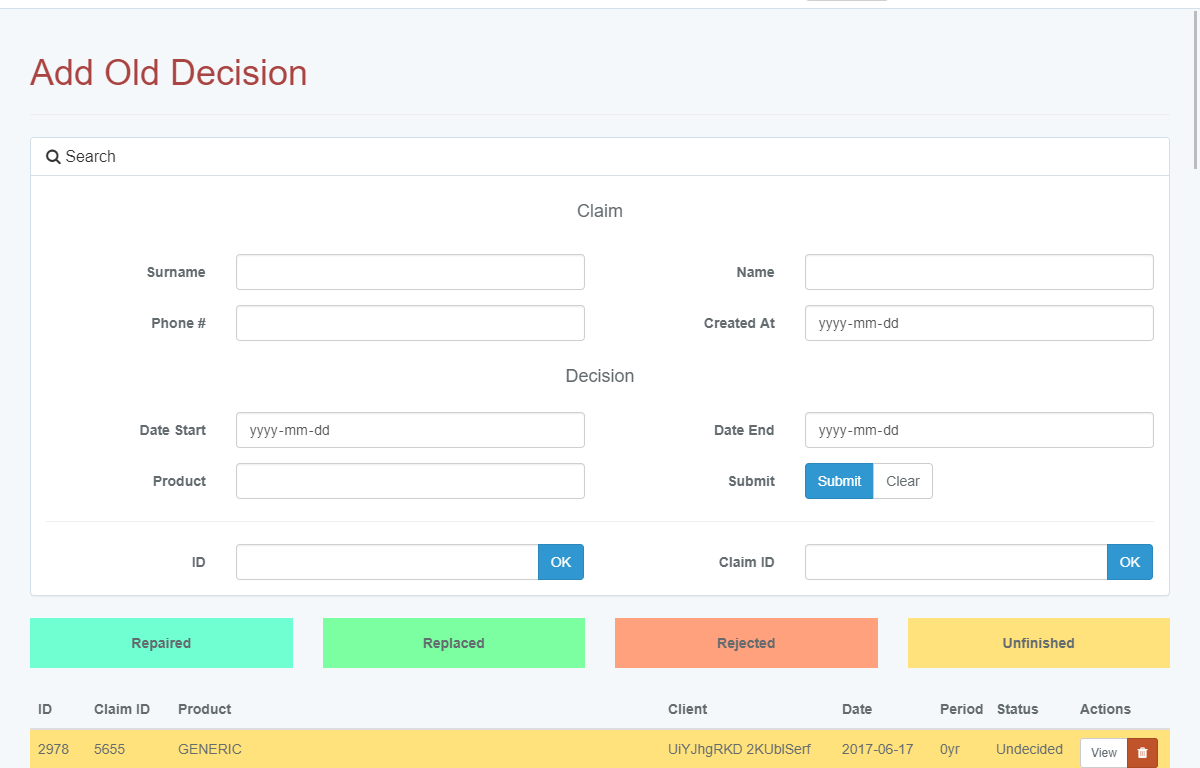
\includegraphics[width=\linewidth]{../imagini/decisions_add_old.png}
			\caption{Interfața de adăugare a unei decizii soluționate anterior}
			\label{fig:decisions_add_old}
		\end{figure}

		\begin{figure}
			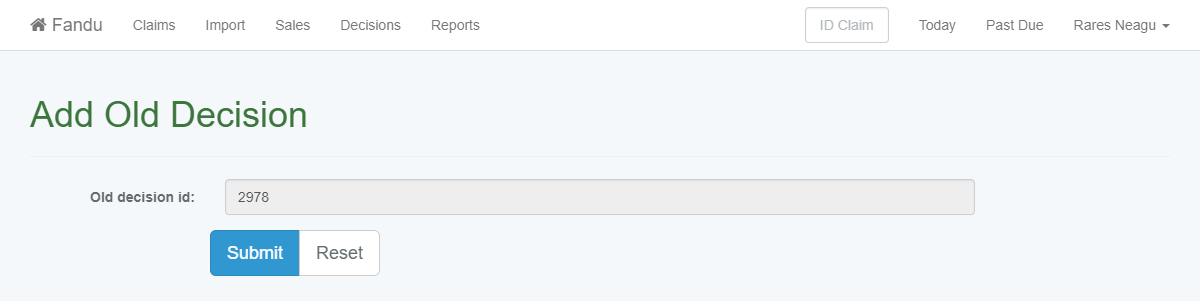
\includegraphics[width=\linewidth]{../imagini/decisions_add_conirm.png}
			\caption{Confirmarea adăugării deciziei soluționate anterior}
			\label{fig:decisions_add_conirm}
		\end{figure}

	\subsection{Modulul de raportări}

		Modulul de raportări se poate accesa prin butonul „Reports” din bara de meniu.

		Fiecare raport poate fi descărcat sau vizualizat în cadrul paginii, alegând „Type” -> „Download” sau „View”.

		Când se alege descărcarea raportului, apare câmpul „Download Type”.
		Sunt valabile următoarele opțiuni:
		\begin{enumerate}
			\item \verb|Excel| - Se va descărca un fișier Excel.
			\item \verb|CSV| - Se va descărca un fișier în formatul \verb|.csv|.
		\end{enumerate}

		Pentru fiecare raport se poate specifica o dată de început și sfârșit a perioadei raportului.

		În cazul în care lipsește data de început, raportul va începe cu prime elemente ale bazei de date până la data de sfârșit.
		În cazul în care lipsește data de sfârșit, se vor include în raport toate elemente de la data de început.
		În cazul lipsei ambelor perioadelor, se generează raportul cu toate datele existente în baza de date.

		În momentul apăsării butonului „Submit”, generarea raportului se va vedea în bara de progres.

		Conform figurii~\ref{fig:reports}, sunt disponibile următoarele rapoarte:
		\begin{enumerate}
			\item \verb|Statistics| - Statistici rapide (câte cereri de despăgubire, decizii au fost create în perioada respectivă de timp).
			Sunt implicit vizualizate în interfața web, precum în figura~\ref{fig:statistics}.
			\item \verb|Decisions| - Raport cu toate deciziile plătite într-o anumită perioada de timp.
			\item \verb|Products| - Raport cu numărul de asigurări, grupate în funcție de tipul de asigurare și prețul ei, în perioada respectivă.
			\item \verb|Sales| - Raport cu numărul vânzărilor asigurărilor grupate în funcție de magazinul ce a făcut vânzarea, împreună cu perioada când s-a vândut primul și ultimul produs.
			\item \verb|Yearly Statistics| - Raport detaliat despre produsele ce încă sunt asigurate, împreună cu posibila cerere de despăgubire asociată.

			Momentan toate asocierile cu cererile de despăgubire trebuie verificate manual, deoarece nu mai sunt corelate vânzările de cererile de despăgubire.
			\item \verb|Monthly Statistics| - Raportul asemănător generat de \verb|Yearly Statistics|, cu câmpul lunii adăugat.
		\end{enumerate}

		\begin{figure}
			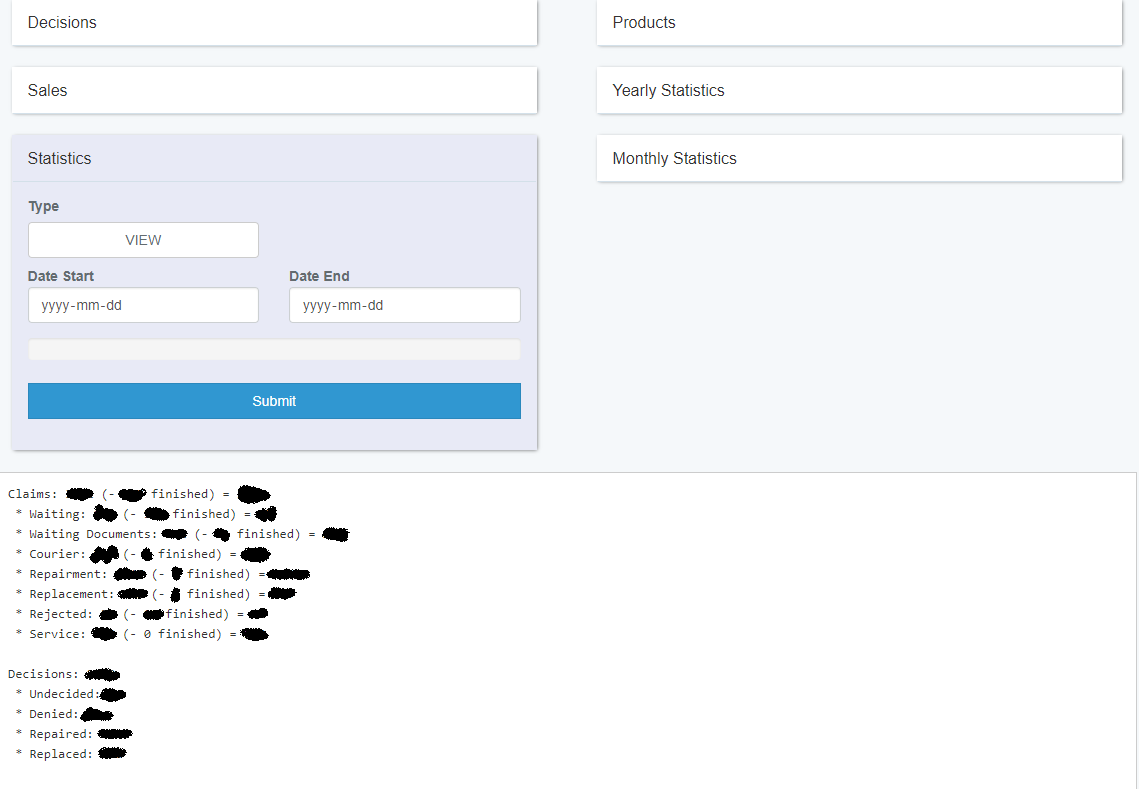
\includegraphics[width=\linewidth]{../imagini/statistics.png}
			\caption{Statistici}
			\label{fig:statistics}
		\end{figure}

		\begin{figure}
			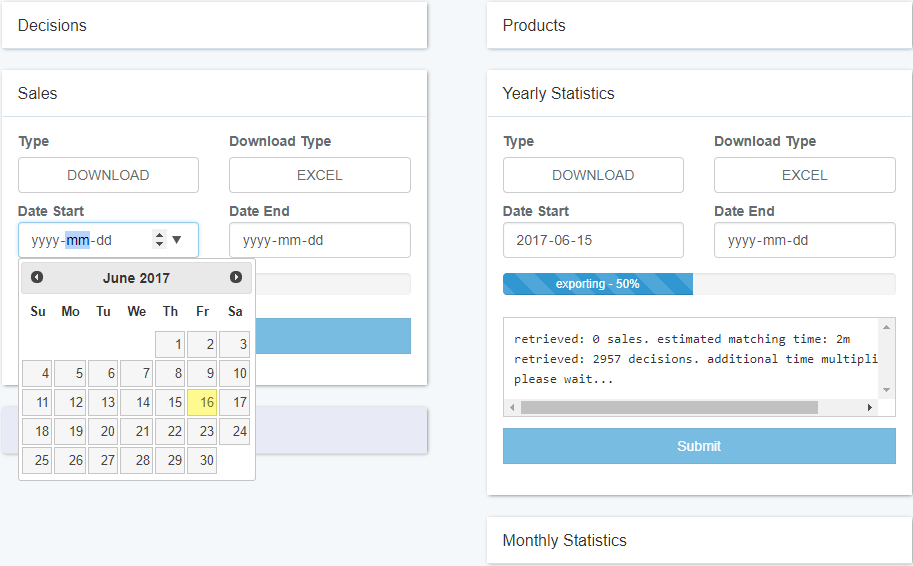
\includegraphics[width=\linewidth]{../imagini/reports.png}
			\caption{Sistemul de raportare}
			\label{fig:reports}
		\end{figure}
